\chapter{Experimental Implementation}
Following the methodological framework outlined in the previous chapter, this section details the concrete experimental implementation of the person-following system. It describes the practical deployment of the software stack, the configuration of the distributed network nodes, and the structural implementation of the control loops. This chapter serves as a comprehensive technical guide, moving from the initial environment setup to the specific programming of the computer vision and navigation nodes.

\section{Development Environment}
To develop and deploy applications within a modern robotics ecosystem, a stable and specialized development environment is paramount. While recent iterations of the Robot Operating System (ROS 2) offer limited compatibility with Windows architectures, the framework is natively designed for and best optimized on Linux distributions. For the implementation of this thesis, ROS 2 Humble Hawksbill was deployed on an Ubuntu 22.04 LTS (Jammy Jellyfish) operating system. Because ROS 2 is primarily managed via command-line interface (CLI) terminal inputs, the core framework operates efficiently without demanding specialized external package managers for its basic management.

The software components—comprising both the custom ROS 2 nodes and the high-level YOLO perception models—were implemented using the Python programming language. Python was selected due to its expressive syntax, object-oriented programming (OOP) support, and its extensive ecosystem of data-science libraries, making it an ideal language for rapid software prototyping in research environments. To ensure software stability and prevent dependency conflicts across the system, a Python Virtual Environment (venv) was established. This isolated container allows for the secure installation and version management of required external modules, including the \texttt{ultralytics} suite for machine learning inference and \texttt{opencv-python} for image matrix manipulation, without altering the global system environment.

To maintain historical records of the codebase, track changes, and facilitate structured development, Git was utilized as the primary version control system in combination with GitHub as the cloud-based repository hosting service. This setup ensured a reliable backup of the source code and allowed for systematic debugging by enabling rollbacks to previous stable software states. For the actual code writing, Visual Studio Code (VSCode) was chosen as the Integrated Development Environment (IDE). 

Managing the distributed architecture required seamless remote access to the TurtleBot 4's onboard Single-Board Computer (SBC). While standard remote administration is achievable through native Secure Shell (SSH) terminal commands, a more integrated approach was chosen by leveraging the VSCode Remote - SSH extension. This extension allows the developer to connect the local IDE directly to the robot's filesystem over the wireless network, streamline real-time code editing, and interact with the robot's environment through a single, unified development interface.

Finally, all custom-developed nodes and configurations described in the subsequent sections of this chapter were organized into a single, dedicated ROS 2 package named \texttt{yolobot}. In the ROS 2 ecosystem, a package serves as the fundamental organizational unit used to bundle software, custom message definitions, launch files, and dependency manifests. By encapsulating the entire implementation within the \texttt{yolobot} package, the project maintains a high degree of modularity, ensuring that the developed person-following pipeline can be easily compiled, transferred, and reused on other ROS 2-compatible robotic systems.

\section{YOLO Detection Node}
The core perception capabilities of the software stack are encapsulated within the \texttt{yolo\_detect} node. Developed as the initial component of the \texttt{yolobot} package, this node is responsible for executing real-time object detection and transforming raw sensory data into structured semantic information. 

Architectural interactions and data flows of this node within the ROS 2 ecosystem are illustrated in Figure~\ref{fig:yolo_node_graph}.

\begin{figure}[!ht]
	\centering
	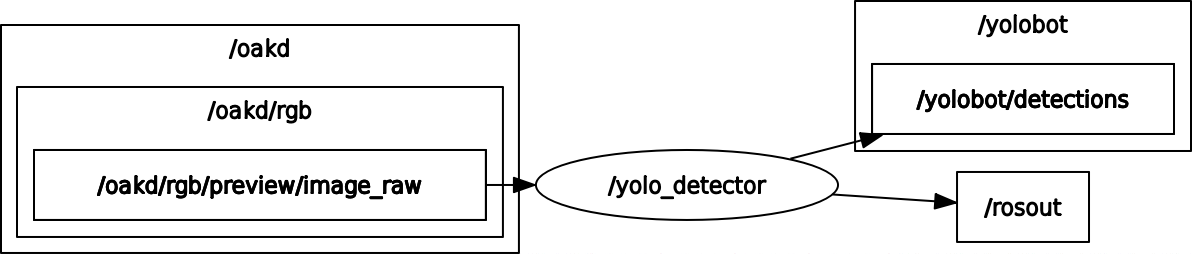
\includegraphics[width=0.8\linewidth]{figures/yolo_detector.png}
	\caption[ROS 2 Node Graph for yolo\_detect]{Computation graph displaying the input image subscription and output bounding box publishers for the yolo\_detector node.}
	\label{fig:yolo_node_graph}
\end{figure}

The functional mechanism of the node relies on an asynchronous callback pipeline. The node subscribes to the raw image telemetry broadcast by the spatial camera on the \texttt{robot7/oakd/rgb\newline/preview/image\_raw} topic. Upon receiving a standardized ROS \texttt{sensor\_msgs/msg/Image} message, the node utilizes the \texttt{cv\_bridge} library to convert the image matrix into a BGR format compatible with OpenCV.

The converted frame is subsequently processed by the YOLO object detection model. To optimize performance and ensure deterministic behavior tailored to this application, the model is configured with a strict confidence threshold ($\tau = 0.8$) and filtered to exclusively retain class ID $0$, which corresponds to the "person" label within the COCO dataset. The model extracts the resulting two-dimensional coordinates of the bounding boxes, populates a standardized \texttt{vision\_msgs/msg/Detection2DArray} message, and publishes the localized metadata to the \texttt{/yolo/detections} topic.

In the early stages of development, the vision pipeline was split across three distinct standalone nodes to decouple verification from data transmission: \texttt{yolo\_basic} managed standard terminal output logs, \texttt{yolo\_viz} published annotated image streams for visual validation, and \texttt{yolo\_detect} handled array publishing. To eliminate software redundancies and reduce network overhead, these variations were refactored into a single, unified node. The core image processing routine is detailed in Listing~\ref{lst:yolo_process}.

\lstinputlisting[linerange={113-134},language=Python,caption={Core image processing and bounding box extraction callback within the unified node.},label={lst:yolo_process}]{codes/yolo_detect.py}

The operational behavior of this consolidated node can be dynamically adjusted at runtime utilizing the native ROS 2 parameter server. By toggling the \texttt{enable\_basic} and \texttt{enable\_viz} parameters respectively, the user can conditionally activate localized logging or video visualization features. The structural implementations of these optional sub-modules are presented in Listings~\ref{lst:yolo_basic} and \ref{lst:yolo_viz}.

\lstinputlisting[linerange={195-204},language=Python,caption={Optional logging logic controlled via the enable\_basic parameter.},label={lst:yolo_basic}]{codes/yolo_detect.py}

\lstinputlisting[linerange={206-221},language=Python,caption={Optional stream annotation and visualization publisher controlled via the enable\_viz parameter.},label={lst:yolo_viz}]{codes/yolo_detect.py}

To ensure seamless deployment across different host machines without requiring absolute file path definitions, the node is engineered to resolve its asset paths dynamically relative to the ROS 2 workspace workspace structure. The neural network weights (\texttt{.pt} files) are allocated a dedicated directory within the share space of the package. During the node's instantiation phase, the path is resolved programmatically, allowing the framework to securely load the model file regardless of the global deployment environment, as demonstrated in Listing ~\ref{lst:yolo_path}.

\lstinputlisting[linerange={45-50},language=Python,caption={Dynamic resolution of the internal package path for model instantiation.},label={lst:yolo_path}]{codes/yolo_detect.py}

\section{Object Localization Node}
The \texttt{object\_locator} node functions as a critical translation and data-fusion layer between the high-level perception pipeline (\texttt{yolo\_detect}) and the downstream navigation state machine. The primary responsibility of this node is to project two-dimensional bounding box coordinates into accurate three-dimensional spatial coordinates relative to the robot's reference frame.

The architectural interactions, incoming topic subscriptions, and outgoing data streams for this node are visualized in Figure~\ref{fig:locator_node_graph}.

\begin{figure}[!ht]
\centering
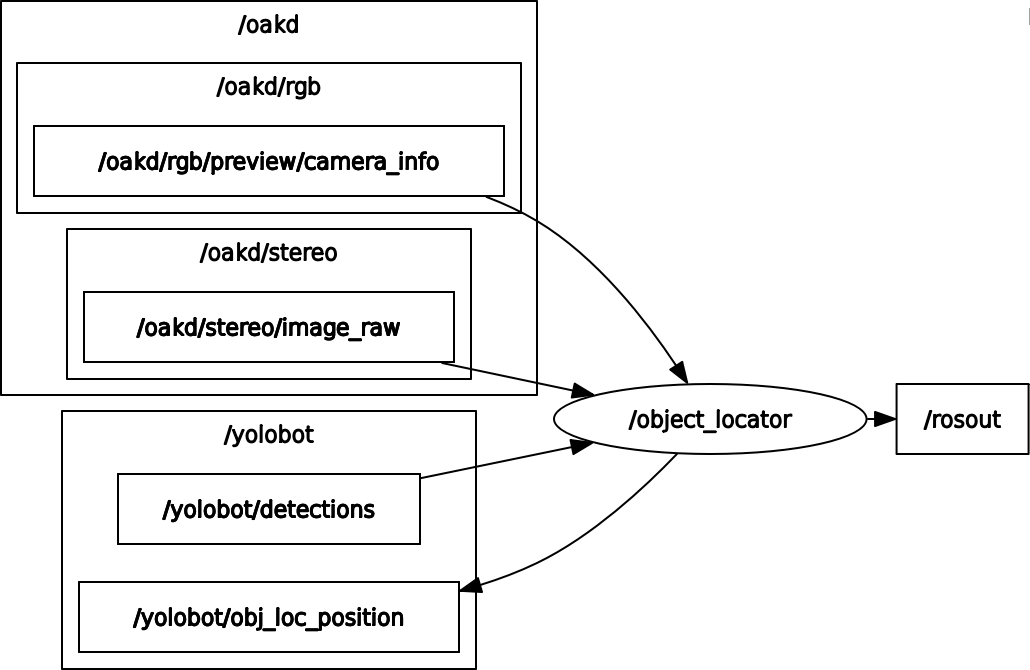
\includegraphics[width=0.8\linewidth]{figures/object_locator.png}
\caption[ROS 2 Node Graph for object\_locator]{Computation graph illustrating the input subscriptions from the YOLO detection node and camera topics, alongside the output spatial coordinate publishers.}
\label{fig:locator_node_graph}
\end{figure}

To perform spatial calculations, the node subscribes to a heterogeneous array of four distinct data streams using standardized ROS~2 interfaces:
\begin{itemize}
\item \textbf{YOLO Detections Sub}: Subscribes to the \texttt{/yolo/detections} topic, ingesting messages of type \texttt{vision\_msgs/msg/Detection2DArray} to receive the bounding boxes from the perception pipeline.
\item \textbf{Camera Info Sub}: Subscribes to the \texttt{/robot7/oakd/rgb/preview/camera\_info} topic using the \texttt{sensor\_msgs/msg/CameraInfo} message type to extract lens intrinsic parameters required for spatial back-projection.
\item \textbf{Stereo Depth Sub}: Subscribes to the \texttt{/robot7/oakd/stereo/image\_raw} topic using the \newline \texttt{sensor\_msgs/msg/Image} message type to acquire the structured depth matrices calculated by the camera.
\item \textbf{RGB Image Sub}: Subscribes to the \texttt{/robot7/oakd/rgb/preview/image\_raw} topic, also utilizing the \texttt{sensor\_msgs/msg/Image} type, to capture the live color frames for alignment and visualization.
\end{itemize}

By fusing these internal memory variables via an asynchronous callback scheme, the node calculates the absolute Euclidean distance along the camera’s optical axis. This mathematical transformation yields the exact spatial coordinates $(X, Y, Z)$ of the target in meters, which are then continuously published to the \texttt{/yolo/object\_position} topic as a standardized \texttt{geometry\_msgs/msg/PointStamped} message.

While the primary objective of this thesis is human tracking, the localization pipeline was engineered to be highly modular and object-agnostic. Because the localization logic operates independently of the underlying semantic classification, the system can locate any arbitrary object without modifying the core localization algorithm. The only adaptation required to track different entities would be adjusting the class filtering parameters within the preceding \texttt{yolo\_detect} node. This modular separation of concerns justifies the architectural decision to implement localization as a standalone node. Consequently, the \texttt{object\_locator} can be seamlessly repurposed in future applications to publish spatial coordinates of obstacles for collision avoidance, alternative target-tracking algorithms, or be extended to aggregate multi-camera inputs.

%\lstinputlisting[linerange={1-50},language=Python,caption={Spatial back-projection and depth fusion routine within the object\_locator node.},label={lst:locator_process}]{codes/object_locator.py}

Finally, to streamline real-time validation and debugging during experimental testing, a dedicated ROS~2 parameter named \texttt{visual} was integrated into the node configuration, defaulting to a boolean value of \texttt{False}. When a user explicitly toggles this configuration flag to \texttt{True}, an optional visualization sub-module is triggered. This module spins up an additional publisher targeting the \texttt{/yolo/debug\_image} topic with a \texttt{sensor\_msgs/msg/Image} payload. This debug stream overlays the calculated spatial coordinates, distance metrics, and bounding-box targets directly onto the live color frame for visual verification. %An example layout for this visual validation is reserved in Figure~\ref{fig:locator_debug}.

%\begin{figure}[!ht]
%\centering
% \includegraphics[width=0.7\linewidth]{figures/locator_debug_output}
%\caption[Visual Debug Output of the Object Locator]{Example of the generated debug stream displaying spatial coordinate overlays and distance tracking vectors.}
%\label{fig:locator_debug}
%\end{figure}

%\lstinputlisting[linerange={267-361},language=Python,caption={Conditional debug visualization and image publishing logic.},label={lst:locator_debug_code}]{codes/obj_loc.py}

\section{Navigation Integration}
The actuation and path-planning layers of the proposed system are fully integrated into the ROS 2 Navigation (\texttt{Nav2}) ecosystem. Instead of utilizing direct, reactive velocity commands, the TurtleBot 4 leverages advanced global and local planners to safely navigate through human-populated environments. 

The baseline requirement for this navigation pipeline is a static occupancy grid map of the environment. This map is generated prior to the execution of the person-following tasks by manually driving the platform through the operational space while running a Simultaneous Localization and Mapping (\texttt{SLAM}) toolbox. Once completed, the static map is saved and passed down to the \texttt{Nav2} map server. Within this subsystem, global costmaps handle the overall static environment geometry, while local costmaps continuously integrate sensory updates to adapt to transient changes. By building upon this infrastructure, the robot can compute collision-free trajectories, automatically detouring around walls and furniture while maintaining active path planning toward its target destination.

%The computational data flow and node interactions governing this navigation stack are preserved in Figure~\ref{fig:nav_integration_graph}.

%\begin{figure}[!ht]
%	\centering
%	\includegraphics[width=0.8\linewidth]{figures/}
%	\caption[ROS 2 Node Graph for Nav2 Integration]{Computation graph showing the integration of the static map server, localization nodes, and the Nav2 path planners.}
%	\label{fig:nav_integration_graph}
%\end{figure}

% % NOTE: Outcommented listings to prevent compiler errors. Activate when source files are ready.
% \lstinputlisting[linerange={1-30},language=Python,caption={Configuration and initialization scheme for the Nav2 lifecycle nodes.},label={lst:nav2_init}]{codes/navigation_integration.py}


\section{State Machine Implementation}
The decision-making hierarchy and navigational lifecycle of the robot are controlled by a centralized Finite State Machine (\texttt{FSM}). This software node coordinates the overall system behavior by acting as the main interface between the perception pipeline and the \texttt{Nav2} stack. The computational graph and topic layout for the state machine execution are outlined in Figure~\ref{fig:fsm_node_graph}.

\begin{figure}[!ht]
	\centering
	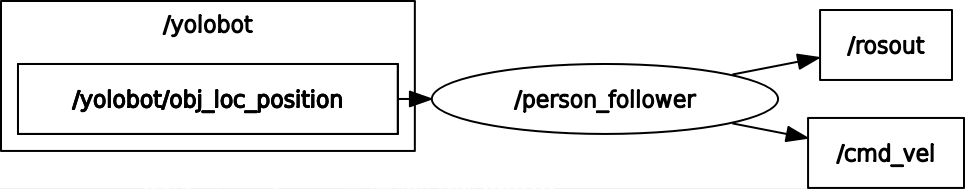
\includegraphics[width=0.8\linewidth]{figures/person_follower.png}
	\caption[ROS 2 Node Graph for the FSM Controller]{Computation graph displaying the transformation of perception topics into Nav2 goal poses controlled via the state machine.}
	\label{fig:fsm_node_graph}
\end{figure}

The state machine node subscribes to the \texttt{/yolo/object\_position} topic to ingest the target's 3D spatial metadata formatted as a \texttt{geometry\_msgs/msg/PointStamped} message. Crucially, because \texttt{Nav2} actions require a definitive target orientation alongside position, the node executes an internal data conversion pipeline. The incoming point data is encapsulated and transformed into a \texttt{geometry\_msgs/msg/PoseStamped} message type, adding default orientation quaternions pointing toward the target. This generated pose is then actively dispatched as a navigational goal to the \texttt{Nav2} action servers.

The operational tracking logic fluidly cycles through five distinct states based on environmental stimuli:
\begin{itemize}
	\item \textbf{\texttt{State.INIT}:} The startup routine responsible for setting baseline software variables and logging initial coordinates, including the robot's physical origin position when docked in its charging dock.
	\item \textbf{\texttt{State.SEARCHING}:} Active when the perception topics yield no detections. The node bypasses the global planner and instructs the base to rotate continuously in place, scanning the environment to discover a person.
	\item \textbf{\texttt{State.FOLLOWING}:} Executed when a valid target is identified. The node continuously intercepts the \texttt{PointStamped} coordinates, transforms them into a \texttt{PoseStamped} format, and forwards these target goals to \texttt{Nav2} to actively navigate toward the moving person.
	\item \textbf{\texttt{State.CLOSE}:} A safety threshold intercept. If the tracking coordinates reveal that the distance to the target falls below a predefined safety margin, the node aborts the current \texttt{Nav2} path execution, halting the TurtleBot 4 to enforce a strict physical buffer zone.
	\item \textbf{\texttt{State.LOST}:} A temporary transitional safety phase triggered upon sudden visual target loss. An internal software timer is immediately spawned. If the human target passes back into the camera's field of view before the timeout expires, the node triggers a smooth transition back into \texttt{State.FOLLOWING}, preventing abrupt stops. If the timer running out confirms a complete target loss, the system reverts to \texttt{State.SEARCHING}.
\end{itemize}

% % NOTE: Outcommented listings to prevent compiler errors. Activate when source files are ready.
% \lstinputlisting[linerange={1-60},language=Python,caption={State machine callback routines, PointStamped-to-PoseStamped conversion, and Nav2 action client dispatch logic.},label={lst:fsm_core}]{codes/state_machine.py}

\section{Testing Procedure}
To evaluate the functional reliability and structural robustness of the integrated software-hardware pipeline, a series of experimental tests was conducted. The primary objective of these procedures was to validate the real-time performance of the detection nodes, the accuracy of the spatial state machine transitions, and the physical safety features of the navigation stack under real-world conditions.

The experimental testing environment was established within a confined indoor space characterized by standard diurnal ambient lighting conditions and unmodified default robotic performance parameters, such as linear and angular velocity limits. Due to its complex spatial geometry and the presence of various arbitrary static obstacles (e.g., household furniture and irregular floor items), this setting provided a highly challenging and realistic proving ground for single-person tracking. This intricate layout allowed for the rigorous evaluation of two critical system capabilities:
\begin{itemize}
	\item \textbf{Dynamic Obstacle Avoidance:} Verifying whether the \texttt{Nav2} local planners could compute collision-free trajectories to bypass tight corners and intervening obstacles while actively pursuing the moving target.
	\item \textbf{Line-of-Sight Occlusion Handling:} Testing the robustness of the \texttt{State.LOST} timer thresholds when the human target was temporarily obscured by spatial architecture or sharp turns.
\end{itemize}

A recognized limitation of this testing procedure was the spatial constraint of the environment. Due to the limited physical dimensions of the room, the maximum operational range and long-distance tracking thresholds of the person-following system could not be fully evaluated. Consequently, comprehensive high-velocity and wide-area benchmarks are reserved for future validation phases.
